
% Asset ID: A21RadiansTikZ-001
% Unit code: A21
% Topic code: A21-TRIG
% Topic ID: A21Radians
% Source: Chapter 5 Radians transcript + P2 Chapter 5 Radians slides
% Related lesson section: Key Definitions and Notation; Core Theory 8.1
% Purpose: Show one radian as the central angle where arc length equals radius.
\documentclass[tikz,border=8pt]{standalone}
\usetikzlibrary{arrows.meta,angles,quotes}
\begin{document}
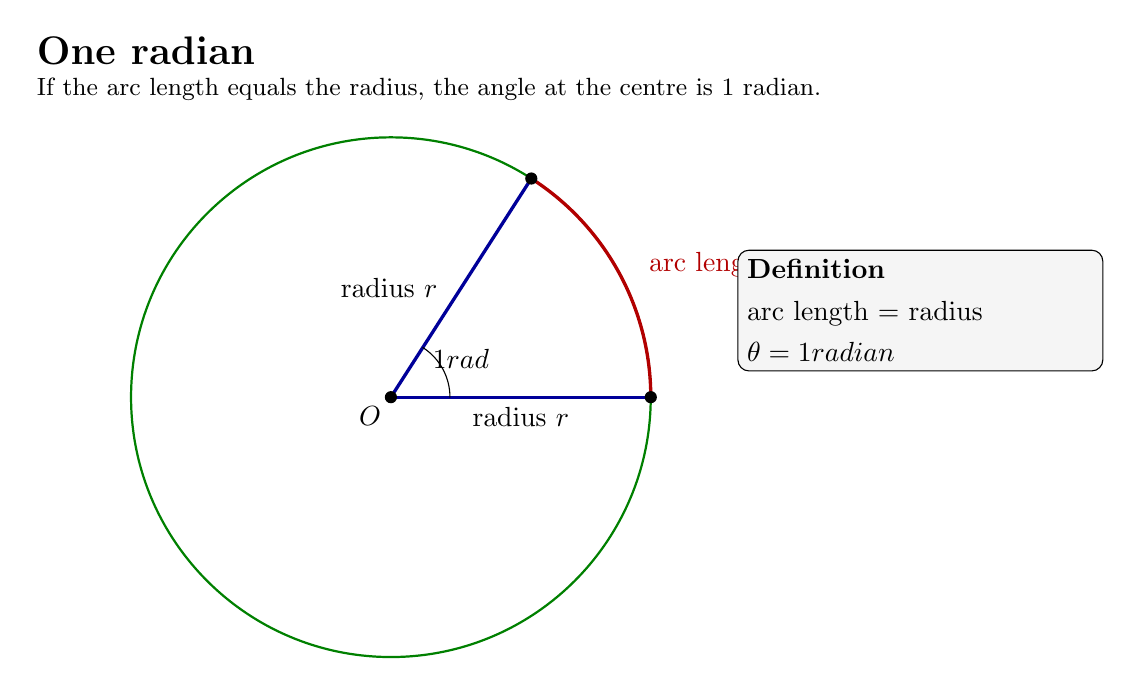
\begin{tikzpicture}[scale=1.1,line cap=round,line join=round]
\def\r{3}\def\ang{57.2958}
\node[anchor=west,font=\bfseries\Large] at (-4.2,4.0) {One radian};
\node[anchor=west,font=\small] at (-4.2,3.55) {If the arc length equals the radius, the angle at the centre is \(1\) radian.};
\draw[green!50!black,thick] (0,0) circle (\r);
\coordinate (O) at (0,0);\coordinate (A) at (\r,0);\coordinate (B) at ({\r*cos(\ang)},{\r*sin(\ang)});
\draw[blue!60!black,very thick] (O)--(A);\draw[blue!60!black,very thick] (O)--(B);
\draw[red!70!black,very thick] (A) arc[start angle=0,end angle=\ang,radius=\r];
\pic[draw=black,angle radius=0.75cm,angle eccentricity=1.35,"$1\text{ rad}$"] {angle=A--O--B};
\fill (O) circle (2pt) node[below left] {\(O\)};\fill (A) circle (2pt);\fill (B) circle (2pt);
\node[below] at (1.5,0) {radius \(r\)};\node[left] at ({1.2*cos(\ang)},{1.2*sin(\ang)+0.25}) {radius \(r\)};\node[right,red!70!black] at ({3.25*cos(28)},{3.25*sin(28)}) {arc length \(r\)};
\node[draw,rounded corners,fill=gray!8,align=left,anchor=west,text width=4.4cm] at (4.0,1.0) {\textbf{Definition}\\[3pt]arc length \(=\) radius\\[3pt]\(\theta=1\text{ radian}\)};
\end{tikzpicture}
\end{document}
